\documentclass{article}

\usepackage[ngerman]{babel}
\usepackage{graphicx}
\usepackage{indentfirst}
\usepackage{hyperref}
\usepackage{geometry}
\usepackage{changepage}
\usepackage{booktabs}
\usepackage{float}
\usepackage{tabulary}
\usepackage{multirow}
\usepackage{caption}
\usepackage{subcaption}

\graphicspath{ {./images/} }
\setlength\parindent{0pt}

\makeatletter
\newcommand{\sectionauthor}[1]{
	{\parindent 0em \large \scshape Autor: #1 \par \nobreak \vspace*{1em}}
	\@afterheading
}
\newcommand{\specification}[3]{
	{\parindent 0.5em \hangindent 3em \hypertarget{spec:#1:#2}{\textbf{/#1#2/}} #3 \par \nobreak \vspace*{0.5em}}
}
\makeatother

\title{Bibliotheksanwendung - Feinspezifikation}
\date{\today\\v1.0}
\author{
	Ivan Charviakou\\
	León Liehr\\
	Mohamad Najjar\\
	Jonas Picker\\
	Sergei Pravdin
}

\begin{document}
\maketitle
\begin{figure}[h]
	\centering
	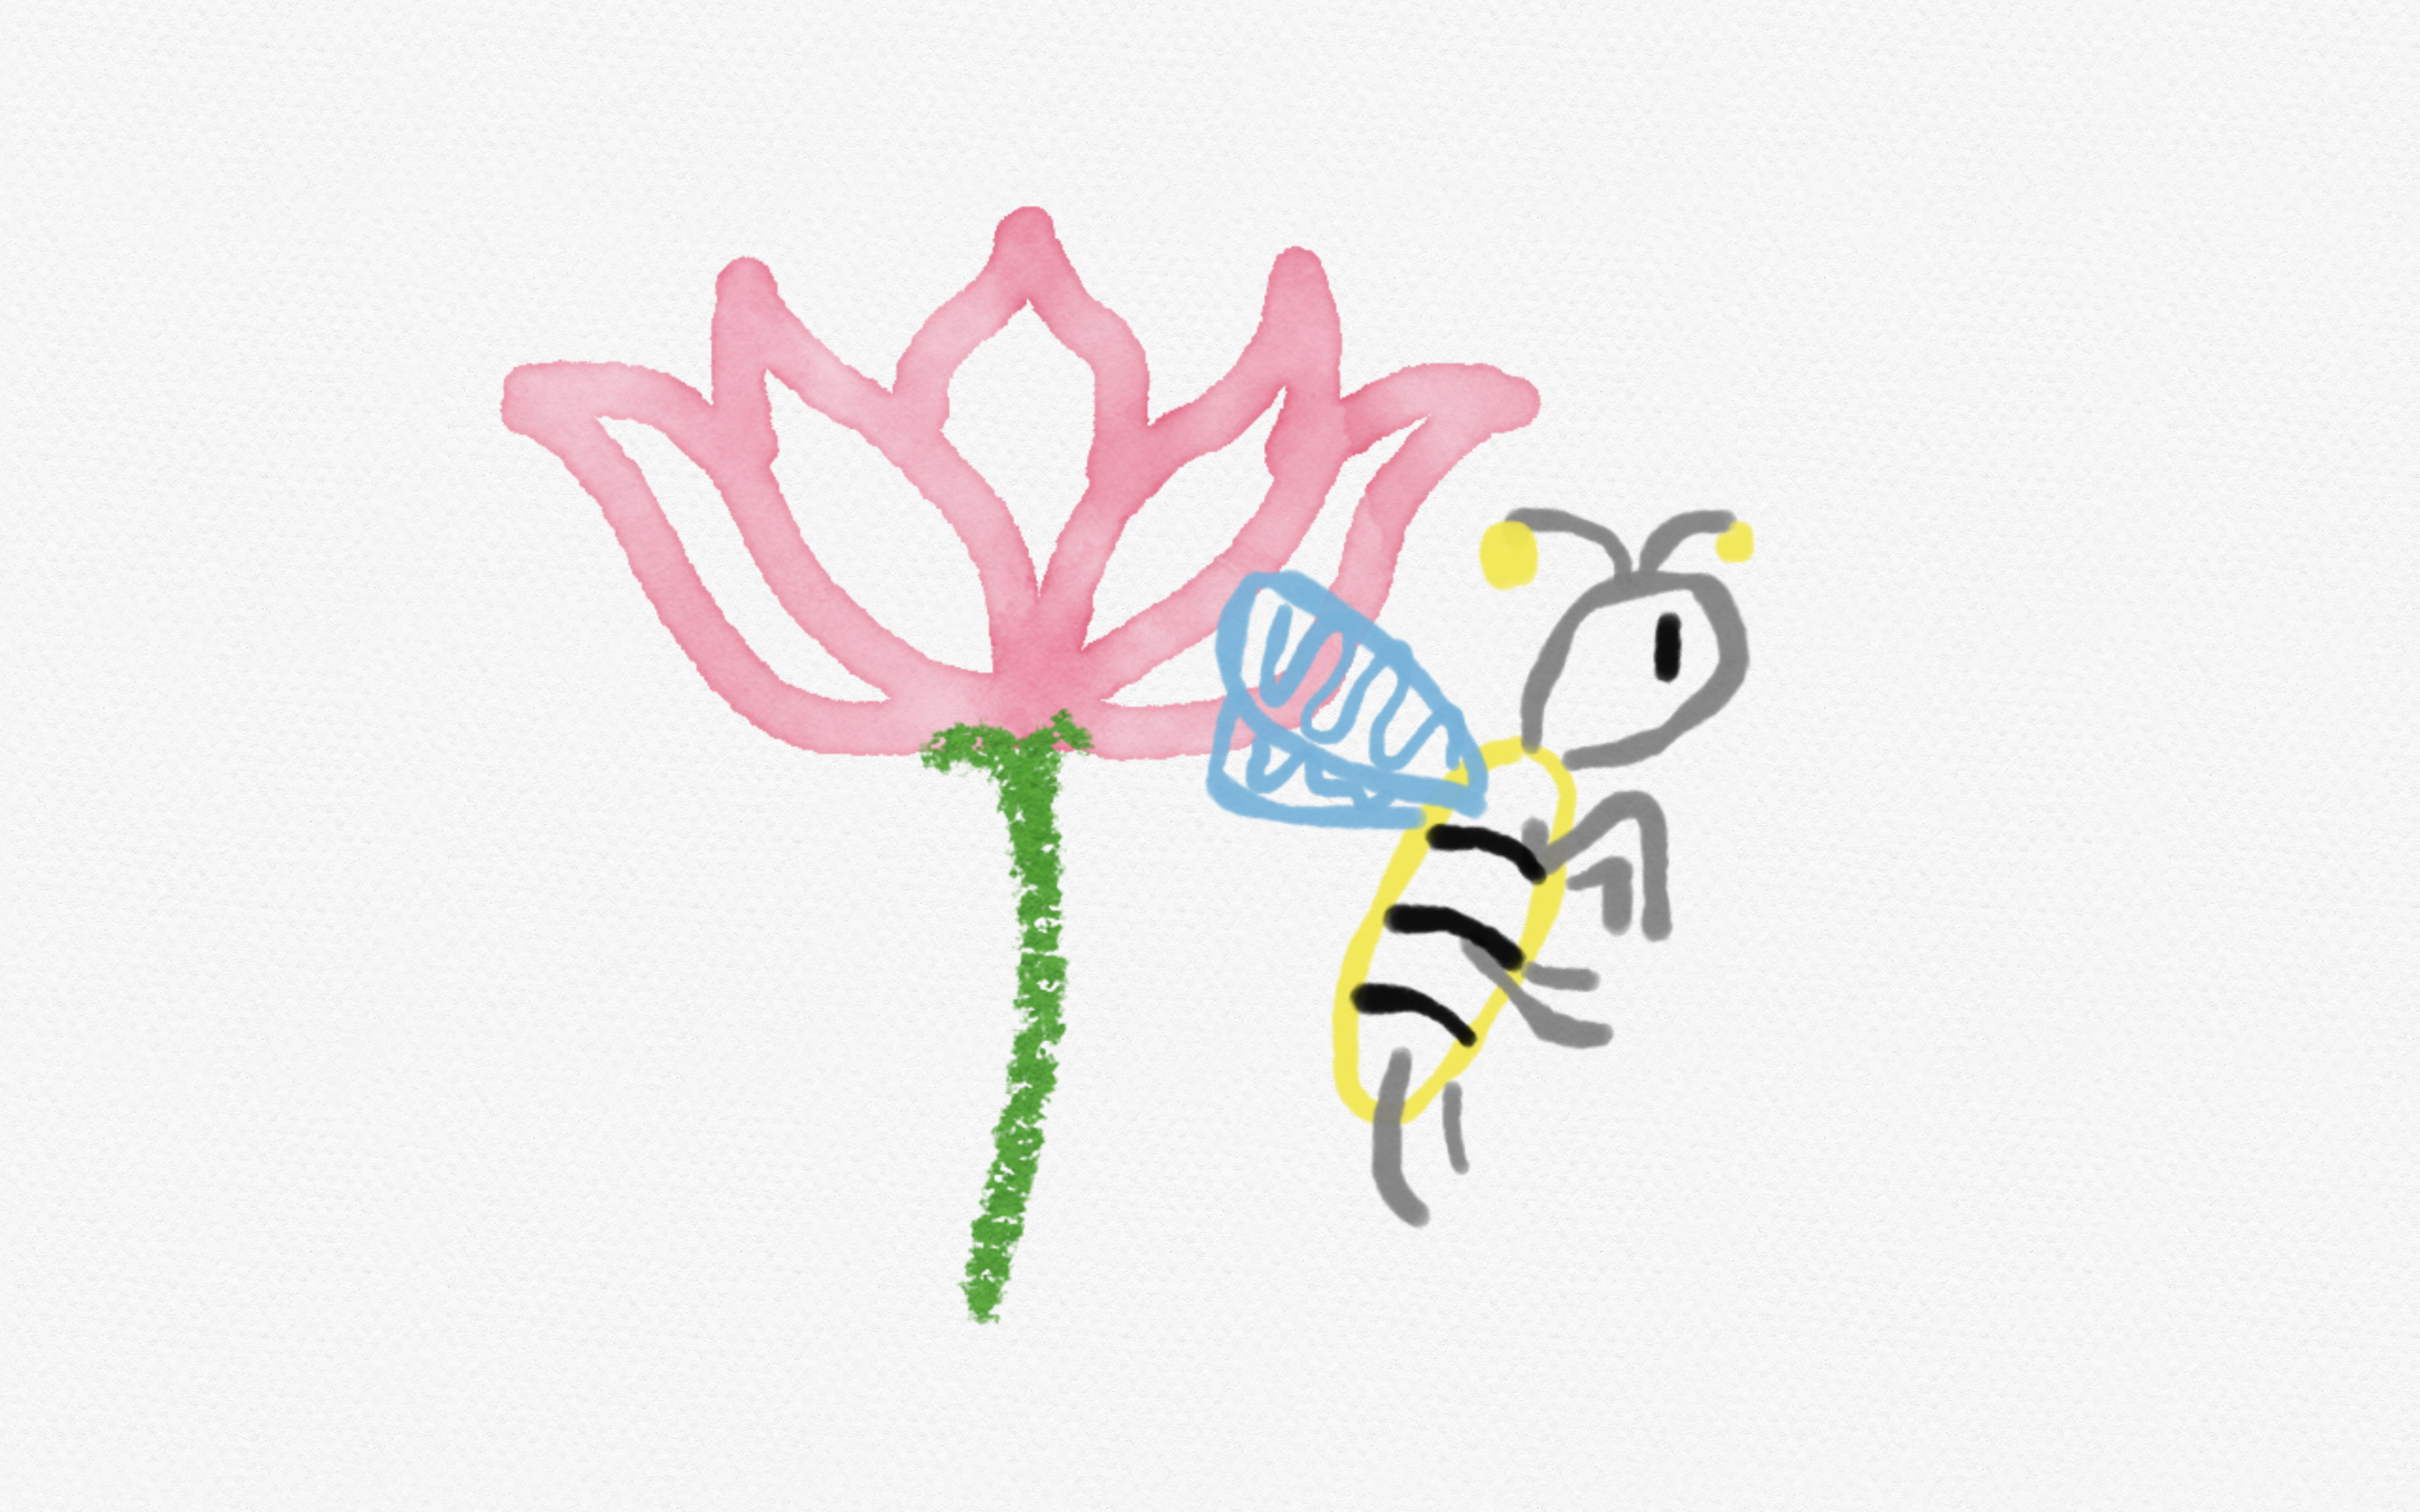
\includegraphics[width = 30em]{Logo}
\end{figure}
\newpage
\tableofcontents
\newpage

%----------------------------------------------------------------------Kapitel 1--------------------------------------------------------------------------------------------

\section{Einleitung}
Bei diesem Dokument handelt es sich um die Feinspezifikation unseres Bibliothekssystems. Es baut direkt auf dem vorangegangenen Entwurf auf und enthält einen noch genaueren Umriss der zu erstellenden Applikation.

%----------------------------------------------------------------------Kapitel 2--------------------------------------------------------------------------------------------

\section{Projektübersicht}
\sectionauthor{Ivan Charviakou}

\subsection{Paketübersicht und Ordnerstruktur}
Das angegebene Diagramm stellt die MVC-Architektur mit den Beziehungen zwischen den einzelnen Komponenten anhand der gegebenen Applikation dar.
Dabei folgt die Komponentenaufteilung der Paketstruktur der Applikation und es werden die Paketnamen zusammen mit den wichtigsten darin enthaltenen Klassen / Komponenten / Funktionalitäten angegeben.
Zudem entsprechen die Farben, die die Pakete im Diagramm besitzen, den Farben im nachfolgenden Klassendiagramm. \vspace{0.5em}

Die Ordnerstruktur des Projekts wird als Ordnerbaum dargestellt.
Während die Paketstruktur im Ordner 'BiBi.src.main.java' abgebildet ist, enthält 'BiBi.src.main.webapp.view' die verwendeten Facelets mit entsprechender Rollenzuordnung. \vspace{0.5em}

\begin{figure}[ht]
	\centering
	\begin{subfigure}[b]{0.45\textwidth}
		\centering
		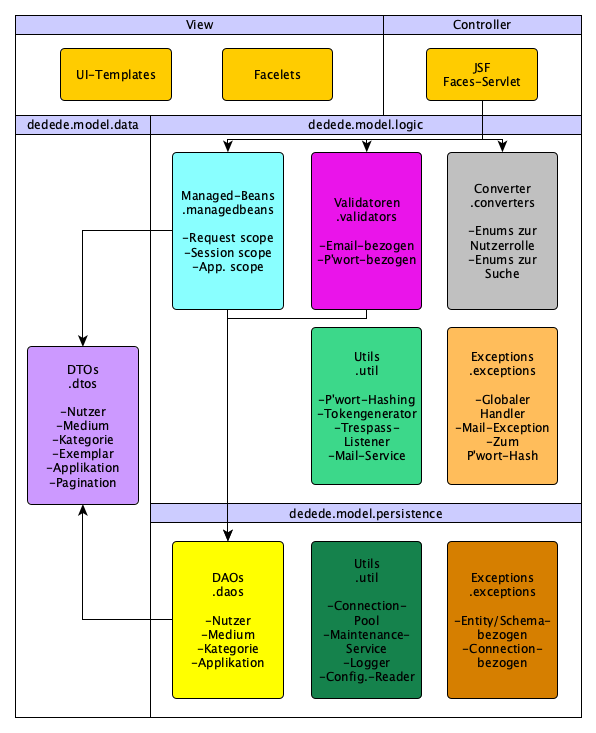
\includegraphics[width = 19em]{Modeldiagramm}
		\caption{Modeldiagramm}
	\end{subfigure}
	\hfill
	\begin{subfigure}[b]{0.45\textwidth}
		\centering
		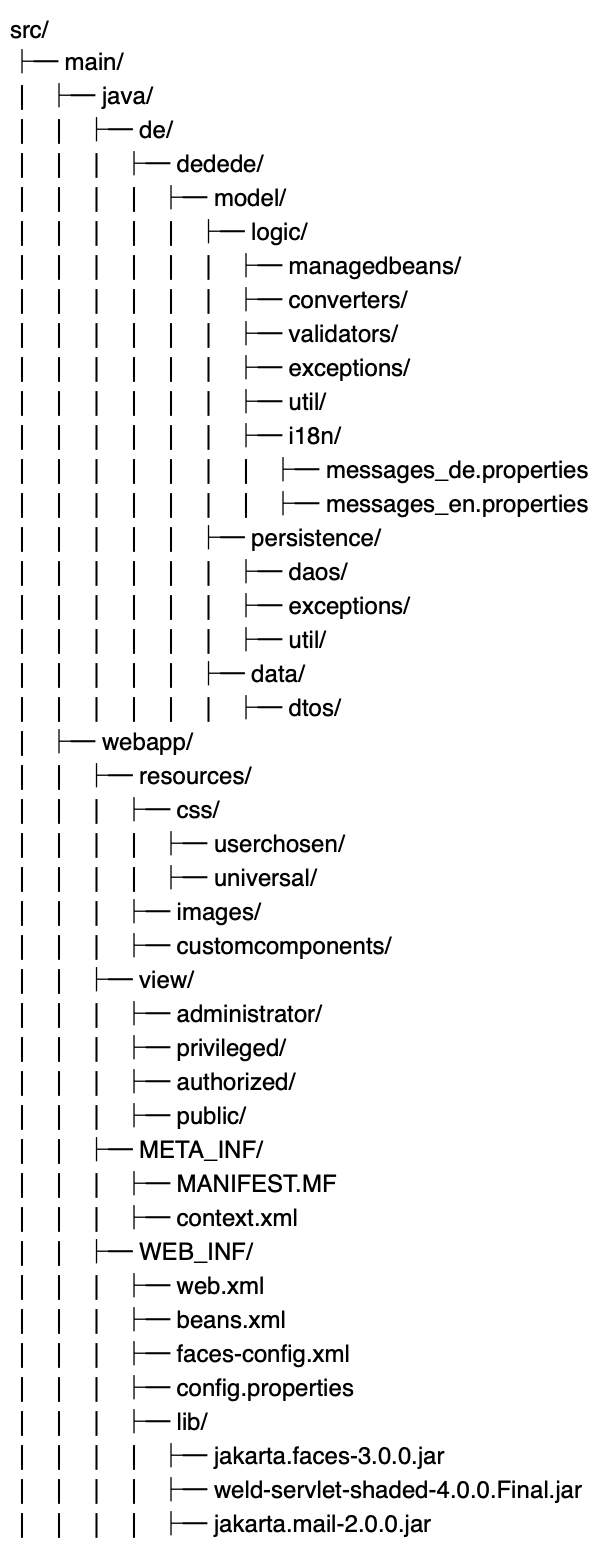
\includegraphics[width = 15em]{FileStructure}
		\caption{Ordnerstruktur}
	\end{subfigure}
\end{figure}

%----------------------------------------------------------------------Kapitel 3--------------------------------------------------------------------------------------------
\section{UML-Klassendiagramm}
\sectionauthor{Mohamad Najjar}
\section{Paketdiagramm}
Das Paketdiagramm veranschaulicht die  Rollen und Beziehungen der Pakete in Ordnerstruktur, als Legende dient es für die im Klassendiagramm verwendeten Farben.


 
    \begin{center}
    \begin{figure}
        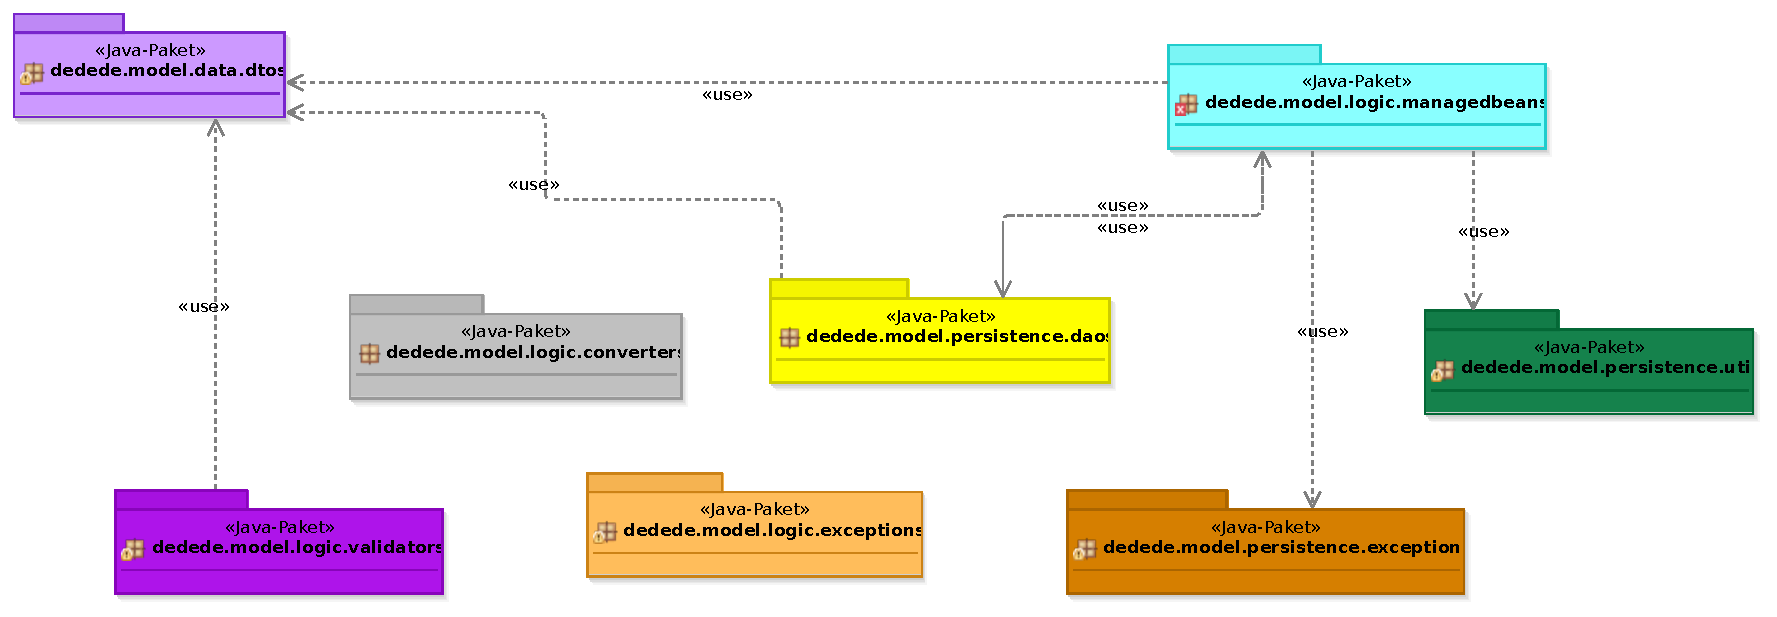
\includegraphics[scale=0.6]{Paketdiagramm.pdf}
        \caption{Paketdiagramm}
        \label{fig:Paketdiagramm}
    \end{figure}
    \end{center}


%----------------------------------------------------------------------Kapitel 4--------------------------------------------------------------------------------------------
\newpage
\section{Bibliotheken}
\sectionauthor{Sergei Pravdin}

\newenvironment{controls}
{
    \begin{table}[H]
        \centering
        \begin{tabular}{ p{7em} p{19em} p{4em} p{12em} }
            \toprule
            \textbf{Bibliothek} & \textbf{Anwendungsbereich} & \textbf{Version} & \textbf{Lizenz}\\
            \midrule
        }
        {
            \bottomrule
        \end{tabular}
    \end{table}
}

Folgende Bibliotheken bzw. Frameworks werden für die Entwicklung unseres Bibliothekssystems verwendet.

\begin{controls}
    Jakarta Server Faces (JSF) & Grafische Benutzeroberflächen des Bibliothekssystems & 3.0.0 & GNU GPL / Java Community Process\\
    JDBC-Treiber für PostgreSQL & Integration des Bibliothekssystems mit der Datenbank & 42.2.20 & GNU GPL / Java Community Process\\
    Apache Tomcat & Webserver & 10.0.2 & Apache-Lizenz 2.0\\
    Weld & Dependency Injection mittels Annotationen & 4.0.1 & Apache-Lizenz 2.0\\
    Jakarta Mail & Senden und Empfangen von E-Mails für die Verifizierung der Nutzers & 1.6.5 & CDDL 1.0, GPL 2.0, BSD\\
    Bootstrap & Anordnung der Frontend-CSS-Komponenten & 5.0.0 & MIT-Lizenz\\
\end{controls}

%----------------------------------------------------------------------Kapitel 5--------------------------------------------------------------------------------------------


%----------------------------------------------------------------------Kapitel 6--------------------------------------------------------------------------------------------


\section{View}
\sectionauthor{León Liehr}

\newcommand{\M}[1]{\texttt{#1}} % monospaced
\newcommand{\tag}[2]{\M{#1:#2}} % JSF tag
\newcommand{\B}[1]{\#\{#1\}} % JSF binding
\newcommand{\MB}[1]{\M{\B{#1}}} % monospaced JSF binding

% @Beacon @Temporary
\newenvironment{controls}
{
    \begin{table}[H]
        \centering
        \begin{tabular}{ p{7em} p{25em} p{7em} }
            \toprule
            \textbf{Typ} & \textbf{Beschreibung} & \textbf{Sichtbarkeit}\\
            \midrule
        }
        {
            \bottomrule
        \end{tabular}
    \end{table}
}

\long\def\begincontrols [#1] #2\endcontrols
{
    \begin{table}[H]
        \centering
        \begin{tabular}{ l l l l }
            \toprule
            & \multicolumn{2}{l}{\textbf{Attribut}} &\\
            \cmidrule(r){2-3}
            \textbf{Typ} & \textbf{Name} & \textbf{Wert} & \textbf{Sichtbarkeit}\\
            \midrule
            #2
            \bottomrule
        \end{tabular}
        \caption{\M{#1.xhtml}}
    \end{table}
}

\newcommand{\PUB}{jeder}
\newcommand{\ANO}{Anon.}
\newcommand{\USR}{Nutzer}
\newcommand{\BIB}{Mitarbeiter}
\newcommand{\ADM}{Admin.}

\newcommand{\component}[2]{\subsubsection{#1 (\texttt{#2})}}
\newcommand{\page}[2]{
    \subsubsection{#1}
    \paragraph*{Dateipfad} \texttt{#2.xhtml}
}

\newcommand{\Javadoc}{\paragraph*{Javadoc}}
\newcommand{\Parameter}{\paragraph*{Parameter}}

\newcommand{\BTN}{\tag{h}{commandButton}}
\newcommand{\LNK}{\tag{h}{outputLink}}
\newcommand{\INP}{\tag{h}{inputText}}
\newcommand{\PAS}{\tag{h}{inputSecret}}
\newcommand{\DRP}{\tag{h}{selectOneMenu}}
\newcommand{\CHK}{Checkbox}
\newcommand{\OUT}{\tag{h}{outputText}}
\newcommand{\LST}{paginierte Liste}

\subsection{Komponenten}

JSF Composite Components.

\subsection{Seitenvorlage}\label{page_template}

JSF Templates.

\begincontrols[template]
    \tag{ui}{insert} & \M{name} & \M{title} & \\
    \tag{ui}{insert} & \M{name} & \M{content} & \\
    \tag{ui}{include} & \M{src} & \hyperref[page_header]{\M{header.xhtml}} & \\
    \tag{h}{messages} & \M{globalOnly} & \M{true} & \\
    \tag{ui}{include} & \M{src} & \hyperref[page_footer]{\M{footer.xhtml}} & \\
\endcontrols

\subsubsection{Kopfzeile}\label{page_header}

\begincontrols[header]
    \multirow{2}{*}{\tag{h}{commandButton}} & \M{id} & \M{xxx} & \\
    & \M{action} & \MB{header.displayHelpText()} & \\
    \INP & \M{value} & \MB{header.mediumSearchTerm} & \\
    \LNK & \M{value} & \M{medium-search.xhtml} & \\
    \tag{h}{graphicImage} & \M{value} & \MB{header.application.logo} & \\
    \OUT & \M{value} & \MB{header.application.name} & \\
    \tag{h}{commandLink} & \M{action} & \MB{header.logOut()} & \\
    \LNK & \M{value} & \M{login.xhtml} & \\
    \LNK & \M{value} & \M{registration.xhtml} & \\
    \LNK & \M{value} & \M{profile.xhtml?id=\B{header.user.id}} & \\
\endcontrols

\subsubsection{Fußzeile}\label{page_footer}

\begincontrols[footer]
    \LNK & \M{value} & \M{privacy-policy.xhtml} & \\
    \LNK & \M{value} & \M{site-notice.xhtml} & \\
    \LNK & \M{value} & \M{contact.xhtml} & \\
\endcontrols

\subsection{Seiten}

\page{Abzuholende Exemplare}{staff/copies-ready-for-pickup}

\Javadoc
This page is used by library staff to be up to speed regarding which copies are ready to be picked up and
whether they can expect someone to soon enter the library and arrive at their counter.

\begin{controls}
    \LST & aller abzuholenden Exemplare & \BIB\\
\end{controls}

\begin{table}[H]
    \centering
    \begin{tabular}{ p{6em} p{6em} p{19em} p{7em} }
        \toprule
        \textbf{Spalte} & \textbf{Typ} & \textbf{Beschreibung} & \textbf{Sichtbarkeit}\\
        \midrule
        Exemplar & \LNK & die Signatur eines Exemplars; zur Direktausleihe & \BIB\\
        Medium & \LNK & Medienattribut mit der Medienvorschauposition Titel; zur Mediensansicht & \BIB\\
        Nutzer & \OUT & E-Mail-Adresse & Nicht-\ADM\\
        Nutzer & \LNK & E-Mail-Adresse; zum Profil & \ADM\\
        Zeit & \OUT & Dauer bis zum Zeitpunkt der Fristüberschreitung & \BIB\\
        \bottomrule
    \end{tabular}
    \caption{Inhalt der paginierten Liste. Jede Zeile existiert pro Exemplar und Nutzer}
\end{table}

\page{Eigene abzuholende Exemplare}{account/my-copies-ready-for-pickup}

\Javadoc
On this page a user gets to know which copies they want to pick up from the library and borrow thereafter
and how much time they have left to do so until they exceed the lending period.

\begin{controls}
    \LST & aller abzuholenden Exemplare & \USR\\
\end{controls}

\begin{table}[H]
    \centering
    \begin{tabular}{ p{6em} p{6em} p{27em} }
        \toprule
        \textbf{Spalte} & \textbf{Typ} & \textbf{Beschreibung}\\
        \midrule
        Exemplar & \OUT & die Signatur eines Exemplars\\
        Medium & \LNK & Medienattribut mit der Medienvorschauposition Titel; zur Mediensansicht\\
        Zeit & \OUT & Dauer bis zum Überschreiten der Abholungsfrist\\
        \bottomrule
    \end{tabular}
    \caption{Inhalt der paginierten Liste. Jede Zeile existiert pro Exemplar}
\end{table}

\page{Eigene ausgeliehene Exemplare}{account/my-borrowed-copies}

\Javadoc
This page informs the user which copies they borrowed from the library and how much time they still have left
until they have to return them to not exceed the lending period.

\begin{controls}
    \LST & aller ausgeliehenen Exemplare & \USR\\
\end{controls}

\begin{table}[H]
    \centering
    \begin{tabular}{ p{6em} p{6em} p{27em} }
        \toprule
        \textbf{Spalte} & \textbf{Typ} & \textbf{Beschreibung}\\
        \midrule
        Exemplar & \OUT & die Signatur eines Exemplars\\
        Medium & \LNK & Medienattribut mit der Medienvorschauposition Titel; zur Mediensansicht\\
        Zeit & \OUT & Dauer bis zum Überschreiten der Rückgabefrist\\
        \bottomrule
    \end{tabular}
    \caption{Inhalt der paginierten Liste. Jede Zeile existiert pro Exemplar}
\end{table}

\page{Anmeldemaske}{public/login}

\Javadoc
This page is the one users first face when they are not already logged in.
It allows them to log into the system to gain the privilege to borrow copies.
If a logged-in user accesses this page by manually entering its URL, a message is shown instead of the
login form and they get automatically redirected to their profile page.

\begincontrols[public/login]
    \INP & \M{value} & \MB{login.user.email} & \ANO\\
    \PAS & \M{value} & \MB{login.user.password} & \ANO\\
    \BTN & \M{action} & \MB{login.logIn()} & \ANO\\
    \tag{h}{commandLink} & \M{action} & \MB{login.resetPassword()} & \ANO\\
\endcontrols

\page{Datenschutzerklärung}{public/privacy-policy}

\Javadoc
This page declares the privacy policy of this system.

\begin{controls}
    \OUT & für die Datenschutzerklärung & Nicht-\ADM\\
    \INP & für die Datenschutzerklärung & \ADM\\
    \BTN & zum Speichern der Änderungen & \ADM\\
\end{controls}

\page{Direktausleihe}{staff/direct-lending}

\Parameter
Optional \texttt{copy}: Signatur eines Exemplars. Füllt das erste Signatureingabefeld.

\Javadoc
This page enables staff to lend a person most probably in front of their counter a series of copies.
It is intended but not a hard requirement that library staff scans the copies given to them by the customer with a dedicated device which automatically pastes the signatures into the corresp. input fields. Analogously with the email address stored inside of their membership card.

\begincontrols[staff/reactive-lending]
    \tag{bibi}{reactiveInputText} & \M{value} & \MB{directLending.borrowingUser.email} & \BIB\\
    % BEACON TASK 5x vorhanden!!!!!
    \tag{bibi}{reactiveInputText} & \M{value} & \MB{COPY.signature} & \BIB\\
    \BTN & \M{action} & \MB{directLending.addSignatureInputField()} & \BIB\\
    \BTN & \M{action} & \MB{directLending.lendMedium()} & \BIB\\
\endcontrols

\page{E-Mail-Bestätigung}{public/email-confirmation}

\Parameter
Optional \texttt{token}.

\Javadoc
Accessing this page potentially verifies the email address of a specific user. For this,
it takes a token as a query parameter. If absent or invalid, nothing user-facing happens.
This secures against certain attacks.

\page{Fehlerseite}{public/error}

\Javadoc
The sink for all kinds of fatal errors that happened in the system.
They are either caused client-side (HTTP status codes 4XX) or server-side (HTTP status codes 5XX).
If it's a client-side error, the user gets redirected to either the login page or their profile depending on if they are logged in or not. The redirection happens after some fixed amount of time.

\begin{controls}
    \OUT & für den Titel der Fehlermeldung & \PUB\\
    \OUT & für die Beschreibung des Fehlers & \PUB\\
\end{controls}

\page{Impressum}{public/site-notice}

\Javadoc
This page contains the site notice.

\begincontrols[public/site-notice]
    % TASK readonly for users and staff
    \INP & \M{value} & \MB{siteNotice.application.siteNotice} & \ADM\\
    \BTN & \M{action} & \MB{siteNotice.save()} & \ADM\\
\endcontrols

\page{Kategorienbearbeitung}{staff/category-editor}

\Parameter
Entweder \texttt{id}: Kennung der zu bearbeitenden Kategorie.
Oder \texttt{parent-id}: Kennung der Elterkategorie, unter welcher eine neue Kategorie erstellt werden soll.

\Javadoc The category editor allows the creation and modification of a category.
Generally this page is accessed from the category browser:
In case the library staff clicks on the edit button next to a category's name in the browser, the corresp. identifier will be transmitted as the Parameter \texttt{id}.
In the other case, it's the create button in the context of a category and the parameter is \texttt{parent-id}.
If the parameters are invalid, the user will be redirected to the error page.

\begincontrols[staff/category-editor]
    \INP & \M{value} & \MB{categoryEditor.category.name} & \BIB\\
    \INP & \M{value} & \MB{categoryEditor.category.description} & \BIB\\
    \BTN & \M{action} & \MB{categoryEditor.save()} & \BIB\\
\endcontrols

\page{Kategorierenstöberer}{public/category-browser}

\Javadoc
This page offers users to browse through all available categories mediums are part of in a structured manner.
It renders it possible for the consumer to discover new mediums.

\begin{controls}
    R. \INP & für den Suchterm der Kategoriensuche & \PUB\\
    \BTN & zum Durchführung der Suche & \PUB\\
    Baumansicht & mancher Kategorien & \PUB\\
    \OUT & für den Namen der ausgewählten Kategorie & \PUB\\
    \OUT & für die Beschreibung der ausgewählten Kategorie & \PUB\\
    \LNK & zur Kategorienbearbeitung & \BIB\\
    \BTN & zum Löschen der Kategorie; zur Elterkategorie & \BIB\\
    \LNK & zur Medienerstellung unter der aktuellen Kategorie & \BIB\\
    \LST & aller Medien (Medienvorschauen) in der ausgewählten Kategorie; je ein \LNK zur Medienansicht & \PUB\\
    \LNK & zur Kategorienbearbeitung (Erstellung einer neuen) & \BIB\\
\end{controls}

\page{Kontakt}{public/contact}

\Javadoc The contact page allows any user to get to know how to contact the site owners.

\begincontrols[public/contact]
    % TASK readonly for users and staff
    \INP & \M{value} & \MB{contact.application.contactInfo} & \ADM\\
    \BTN & \M{action} & \MB{contact.save()} & \ADM\\
\endcontrols

\page{Leihfristverstöße}{admin/lending-period-violations}

\Javadoc
This page displays a list of copies which haven't been returned yet together with the assoc. user who exceeded the lending period.

\begin{controls}
    \LST & von Exemplaren und Nutzern & \ADM\\
\end{controls}

\begin{table}[H]
    \centering
    \begin{tabular}{ p{6em} p{6em} p{27em} }
        \toprule
        \textbf{Spalte} & \textbf{Typ} & \textbf{Beschreibung}\\
        \midrule
        Exemplar & \LNK & die Signatur eines Exemplars; zur Medienrückgabe\\
        Medium & \LNK & Medienattribut mit der Medienvorschauposition Titel; zur Mediensansicht\\
        Nutzer & \LNK & E-Mail-Adresse; zum Profil\\
        Überschreitung & \OUT & Dauer seit dem Zeitpunkt der Fristüberschreitung\\
        \bottomrule
    \end{tabular}
    \caption{Inhalt der paginierten Liste. Jede Zeile existiert pro Exemplar und Nutzer}
\end{table}

\page{Medienerstellung}{staff/medium-creation}

\Parameter
Optional \texttt{category}: Kategorie, unter welcher das Medium erstellt werden soll. Füllt das entsprechende Feld.

\Javadoc
This page allows staff and administrators to add new mediums.

\begincontrols[staff/medium-creation]
    % TASK pro medienattribut
    \INP & \M{value} & \MB{ATTRIBUTE} & \BIB\\
    \INP & \M{value} & \MB{mediumCreation.medium.category} & \BIB\\
    \INP & \M{value} & \MB{mediumCreation.medium.returnPeriod} & \BIB\\
    \INP & \M{value} & \MB{mediumCreation.copy.location} & \BIB\\
    \INP & \M{value} & \MB{mediumCreation.copy.signature} & \BIB\\
    \BTN & \M{action} & \MB{mediumCreation.create()} & \BIB\\
\endcontrols

\page{Medienrückgabe}{staff/return}

\Parameter
Optional \texttt{copy}: Signatur eines Exemplars. Füllt das erste Signatureingabefeld.

\Javadoc
This page enables staff to inform the system that a series of copies were returned to the library, probably right after the user left them at their counter.
It is intended but not a hard requirement that library staff scans the copies given to them by the customer with a dedicated device which automatically pastes the signatures into the corresp. input fields. Analogously with the email address stored inside of their membership card.

\begincontrols[staff/return]
    \tag{bibi}{reactiveInputField} & \M{value} & \MB{return.user.email} & \BIB\\
    % TASK BEACON repeat 5 times (or more)!!!
    \tag{bibi}{reactiveInputField} & \M{value} & \MB{COPY.signature} & \BIB\\
    \BTN & \M{action} & \MB{return.addSignatureInputField()} & \BIB\\
    \BTN & \M{action} & \MB{return.returnMedium()} & \BIB\\
\endcontrols

\page{Mediensuche}{public/media-search}

\Parameter
Optional \texttt{query}: Suchterm.

\Javadoc
This page permits users to search for mediums given some of their attributes as search criteria.
Further, a user can search mediums by category and by the signature of one of their copies.
The page has an optional query parameter corresponding to the search term.
If it is not provided, nothing will be searched and the paginated list of results will not be displayed at all.

\begincontrols[public/medium-search]
    \INP & \M{value} & \MB{mediumSearch.generalSearchTerm} & \PUB\\
    \BTN & \M{action} & \MB{mediumSearch.search()} & \PUB\\
    % TASK three times, converter, grouped
    \DRP & \M{value} & \MB{QUERY.operator} & \PUB\\
    % TASK three times, converter, grouped
    \DRP & \M{value} & \MB{QUERY.criterion} & \PUB\\
    % TASK three times, grouped
    \INP & \M{value} & \MB{QUERY.term} & \PUB\\
    \BTN & \M{action} & \MB{mediumSearch.addNuancedSearchQuery())} & \PUB\\
    % BEACON TEMPORARY
    \LST & & aller Suchergebnisse (als Medienvorschauen); je ein \LNK zur Medienansicht; nur sichtbar, wenn schon gesucht wurde & \PUB\\
\endcontrols

\page{Mediumsansicht}{public/medium}

\Parameter
Zwangsweise \texttt{id}: Kennung des anzuzeigenden Mediums.

\Javadoc
This page provides information about a specific medium and their copies available in the library.
Here, users can borrow a copy by committing themselves to pick up the copy from a library site and actually borrowing it there. To trigger the procedure, they can either click on the pick-up button next to a specific copy or on an isolated button which selects an available copy at random.
If the parameter is missing, the user will be redirected to the medium search page.

\begin{controls}
    \LNK & zurück zur Trefferliste / Mediensuche; nur sichtbar, falls der Nutzer von der Suche kommt & \PUB\\
    \OUT & für ein Medienattribut; existiert pro Medienattribut; mehrwertige Attribute durch Komma getrennt angezeigt & \ANO, \USR\\
    \INP & für ein Medienattribut; existiert pro Medienattribut bzw. pro Wert bei mehrwertigen & \BIB\\
    \BTN & zum Hinzufügen eines weiteren Attributeingabefelds; existiert pro Medienattribut & \BIB\\
    \BTN & zum Speichern der Änderungen an den Medienattributen & \BIB\\
    \BTN & zur Bindung an die Abholung des Mediums; nur sichtbar, falls es dem Nutzer erlaubt ist auszuleihen & \USR\\
    \OUT & für die Rückgabefrist; bezieht auch die nutzerbezogene Frist ein, anders als das \INP{} darunter & \USR\\
    \INP & für die Rückgabefrist & \BIB\\
    \BTN & zum Speichern der Änderungen an der Rückgabefrist & \BIB\\
    \LNK & zum Löschen des Mediums; zur zuvor aufgerufenen Seite & \BIB\\
    Tabelle \ref{tableofcopies} & aller Exemplare & \PUB\\
    R. \INP & für den Standort eines neuen Exemplars & \BIB\\
    \INP & für die Signatur eines neuen Exemplars & \BIB\\
    \BTN & zum Erstellen eines Exemplars & \BIB\\
\end{controls}

\begin{table}[H]
    \centering
    \begin{tabular}{ p{6em} p{6em} p{19em} p{7em} }
        \toprule
        \textbf{Spalte} & \textbf{Typ} & \textbf{Beschreibung} & \textbf{Sichtbarkeit}\\
        \midrule
        Standort & \OUT & & \PUB\\
        Standort & \INP & & \BIB\\
        Verfügbarkeit & \OUT & & \PUB\\
        Signatur & \OUT & & \PUB\\
        Signatur & \INP & & \BIB\\
        Aktionen & \BTN & zum Speichern der Änderungen & \BIB\\
        Aktionen & \BTN & zum Löschen & \BIB\\
        Aktionen & \BTN & zum Stornieren einer Abholung & \BIB\\
        Aktionen & \LNK & zur Direktausleihe; nur sichtbar, falls verfügbar & \BIB\\
        Aktionen & \LNK & zur Medienrückgabe; nur sichtbar, falls ausgeliehen & \BIB\\
        Aktionen & \BTN & zur Bindung an die Abholung; nur sichtbar, falls es dem Nutzer erlaubt ist auszuleihen & \USR\\
        \bottomrule
    \end{tabular}
    \caption{Tabelle aller Exemplare als JSF-\texttt{DataTable}. Jede Zeile existiert pro Exemplar}
    \label{tableofcopies}
\end{table}

\page{Mediumschemabearbeitung}{admin/medium-schema-editor}

\Javadoc
On this page, the administrator can adjust the medium schema (the set of attributes of each medium).

\begin{controls}
    \INP & für den Namen eines Attributs; existiert pro Attribut & \ADM\\
    \DRP & für den Typen eines Attributs; existiert pro Attribut & \ADM\\
    \DRP & für die Wertigkeit (ein-, mehrwertig) eines Attributs; existiert pro Attribut & \ADM\\
    \DRP & für die Position in der Medienvorschau; existiert pro Attribut & \ADM\\
    \BTN & zum Löschen eines Attributes; existiert pro Attribut & \ADM\\
    \BTN & zum Hinzufügen eines weiteren Gruppe aus \INP{}ern und \DRP{}n & \ADM\\
    \BTN & zum Speichern der Änderungen & \ADM\\
\end{controls}

\page{Nutzersuche}{admin/user-search}

\Parameter
Optional \texttt{query}: Suchterm.

\Javadoc
This page enables administrators to search for users.
The page has an optional query parameter corresponding to the search term.
If it is not provided, nothing will be searched and the paginated list of results will not be displayed at all.

\begin{controls}
    \INP & für den Suchterm & \ADM\\
    \BTN & zur Durchführung der Suche & \ADM\\
    \CHK & für das Einschränken auf gesperrte Nutzer & \ADM\\
    \LST & aller Suchergebnisse (als Medienvorschauen); je ein \LNK zur Medienansicht; nur sichtbar, wenn schon gesucht wurde & \ADM\\
\end{controls}

\page{Passwortzurücksetzung}{public/password-reset}

\Parameter
Optional \texttt{token}.

\Javadoc
This page is reached by a user when they click on the link they received in an email.
The account is identified through a token passed as parameter.
After submitting the form, the user is not logged into the system yet, they are redirected to the login form.
This secures against certain attacks.
If the token is absent or invalid, nothing user-facing will happen: Clicking the button still means redirection to the login page.

\begincontrols[public/password-reset]
    \multirow{2}{*}{\tag{f}{viewParam}} & \M{name} & \M{token} & \multirow{2}{*}{\PUB}\\
    & \M{value} & \MB{passwordReset.token} & \\
    \PAS & \M{value} & \MB{passwordReset.password} & \PUB\\
    \PAS & \M{value} & \MB{passwordReset.confirmPassword} & \PUB\\
    \BTN & \M{action} & \MB{passwordReset.resetPassword()} & \PUB\\
\endcontrols

\page{Profilseite}{account/profile}

% expand
\Javadoc
This page is either the profile page of the current user or if it is an administrator possibly also
of a user different from the logged-in one.
It allows a user to change their personal information the system stores and it allows administrators to manage other accounts.

\begin{controls}
    \INP & für den Vornamen & \USR\\
    \INP & für den Nachnamen & \USR\\
    \PAS & für das Passwort & \USR\\
    \PAS & zur Bestätigung & \USR\\
    \INP & für die E-Mail-Adresse & \USR\\
    \INP & für den Ort & \USR\\
    \INP & für die PLZ & \USR\\
    \INP & für die Straße& \USR\\
    \INP & für die Hausnummer & \USR\\
    \DRP & für die Nutzerrolle & \ADM\\
    \CHK & zum Sperren des Nutzers & \ADM\\
    \INP & für die Rückgabefrist & \ADM\\
    \BTN & zum Speichern der Änderungen an den Benutzerdaten & \USR\\
    \LNK & zu den abzuholenden und ausgeliehenen Exemplaren & \USR\\
    \BTN & zum Schließen des Accounts; zur Anmeldemaske & \USR\\
    \BTN & zum Löschen des Nutzers; zur Verwaltungsseite & \ADM\\
\end{controls}

\page{Registrierungsseite}{public/registration}

\Javadoc
On this page an anonymous user can register themself. Additionally, it can be used by administrators to register new users.

\begin{controls}
    \INP & für den Vornamen & \ANO/\ADM\\
    \INP & für den Nachnamen & \ANO/\ADM\\
    \PAS & & \ANO/\ADM\\
    \PAS & zur Bestätigung & \ANO/\ADM\\
    \INP & für die E-Mail-Adresse & \ANO/\ADM\\
    \INP & für den Ort & \ANO/\ADM\\
    \INP & für die PLZ & \ANO/\ADM\\
    \INP & für die Straße & \ANO/\ADM\\
    \INP & für die Hausnummer & \ANO/\ADM\\
    \DRP & für die Nutzerrolle & \ADM\\
    \BTN & zum Registrieren des Accounts & \ANO/\ADM\\
\end{controls}

\page{Verwaltungsseite}{admin/administration}

\Javadoc
This page provides the means to administrators to change several global settings of the application.

\begin{controls}
    \INP & für die Rückgabefrist & \ADM\\
    \INP & für den Mahnungszeitpunkt & \ADM\\
    \INP & für die Abholfrist & \ADM\\
    \INP & für den Systemnamen & \ADM\\
    \CHK & für den Zugangsstatus (anonym oder nicht) & \ADM\\
    \CHK & für den Registrierungsstatus & \ADM\\
    \INP & für den regulären Ausdruck valider E-Mail-Adressen & \ADM\\
    \DRP & für das Farbschema des Systems & \ADM\\
    Datei-Upload & für das Logo des Systems & \ADM\\
    \BTN & zum Speichern der Änderungen an den Systemeinstellungen & \ADM\\
    \LNK & zu der Registrierungsseite (fremden Nutzer erstellen) & \ADM\\
    \LNK & zur Mediumsschemabearbeitung & \ADM\\
    \LNK & zu den Leihfristverstößen & \ADM\\
    \LNK & zur Nutzersuche & \ADM\\
    \INP & für den Suchterm einer Nutzersuche & \ADM\\
    \BTN & zum Durchführung der Suche & \ADM\\
\end{controls}

%----------------------------------------------------------------------Kapitel 7--------------------------------------------------------------------------------------------


%----------------------------------------------------------------------Kapitel 8--------------------------------------------------------------------------------------------
\newpage
\section{Datenfluss}
\sectionauthor{Sergei Pravdin}
Die Kommunikation zwischen den Klassen und die Interaktionen des Systems werden durch die Sequenzdiagramme abgebildet. Um einen Datenfluss beispielhaft zu zeigen, werden die folgenden beiden Szenarien vorgelegt: Zuerst bucht ein angemeldeter Nutzer ein Medium-Exemplar erfolgreich zur Ausleihe. Im zweiten Szenario bucht ein angemeldeter Nutzer ein Medium-Exemplar erfolglos zur Ausleihe, weil die Verbindung mit der Datenbank fehlgeschlagen ist. Das System ist so eingestellt, dass die angemeldeten Nutzer Zugriff auf die Medien haben. Der Nutzer möchte ein Exemplar des Mediums 'Programmieren lernen' buchen. Im System existiert das Medium mit dem Titel 'Programmieren lernen' und mit der Signatur (ID) '17RE'. Das Exemplar mit der Signatur (ID) '17RE (+1)' gehört zu dem genannten Medium und ist für eine Buchung verfügbar. Der Nutzer ruft die Mediumsseite 'medium.xhtml?id=17RE' auf.
\subsection{Interaktionen beim erfolgreichen Buchen eines Medium-Exemplars}
\subsubsection{Initialisierung der Mediumsseite}
Beim Laden der Mediumsseite wird zuerst die Methode 'init' als @PostConstruct aufgerufen. Die 'init'-Methode erzeugt ein Medium-DTO, das Medium-DTO hat eine Kollektion der CopyDTOs und eine Kollektion der AttributeDTOs, folglich werden sie vom Medium-DTO erstellt. Der Nutzer bekommt das MediumDTO und setzt eine Medium-ID, die aus dem 'viewParam' zur Verfügung gestellt wird. Danach wird die 'viewAction()' durchgeführt, welche die Mediumsseite durch die statische Methode aus dem Medium-DAO liefern muss. Das Medium-DAO bekommt auf der Persistence-Schicht eine Verbindung von der Singleton-ConnectionPool-Klasse durch die Methoden 'getInstance()' und 'getConnection()'. Im Körper der Methode 'loadMedium' wird eine SELECT-Anfrage durchgeführt, danach gibt das Medium-DAO die Verbindung durch die Methode 'releaseConnection' frei. Das Medium-DAO befüllt mit den von der Datenbank erhaltenen Attributen das Medium-DTO (inkl. CopyDTOs und AttributeDTOs) und gibt es dem Medium-BB zurück. Die Mediumsseite ist nun durch die Methode 'getAttributes' des Medium-DTOs vollständig geladen.
\subsubsection{Buchen eines Exemplars}
Durch die Methode 'getCopies' des Medium-DTOs ist das gewünschte Exemplar für den Nutzer sichtbar. Der Nutzer klickt auf den Buchen-Button des Exemplars. Beim Klicken ruft der Nutzer die Methode 'pickUpAnyCopy' des Medium-BBs auf. Im Körper dieser Methode wird die Methode 'checkAccountStatus()' aus dem UserSession-BB aufgerufen, um zu prüfen, ob der Nutzer Zugriff auf die Funktion Buchen hat. Das UserSession-Bean meldet dem Medium-BB ein positives Ergebnis (OPENED-Status) zurück. Das Medium-BB ruft die statische Methode 'MediumDAO.pickUpAnyCopy(mediumDTO)' auf. Das Medium-DAO bekommt durch die Methoden 'getInstance()' und 'getConnection()' auf der Persistence-Schicht eine Verbindung von der Singleton-ConnectionPool-Klasse. Falls ein availabilityStatus des Exemplars immer noch 'AVAILABLE' ist, wird wird eine UPDATE-Anfrage im Körper der Methode 'loadMedium'  durchgeführt. Im Anschluss gibt das Medium-DAO die Verbindung durch die Methode 'releaseConnection' frei. Als Ergebnis der Methode 'pickUpAnyCopy' bekommt das Medium-BB 'true'. Das Medium-BB vergibt den neuen Status 'MARKEDTOCOLLECT' an das Exemplar. Der Nutzer bekommt eine Nachricht durch die statische Methode 'RessourceBandleHandler.getValue()' und die Buchung ist erfolgreich abgeschlossen. Vom Ressource-Bandle-Handler wird der Nutzer entsprechend benachrichtigt.
\newgeometry{left=0cm,right=0cm,top=0cm,bottom=2cm}
\newpage
\begin{figure}[h]
    \centering
    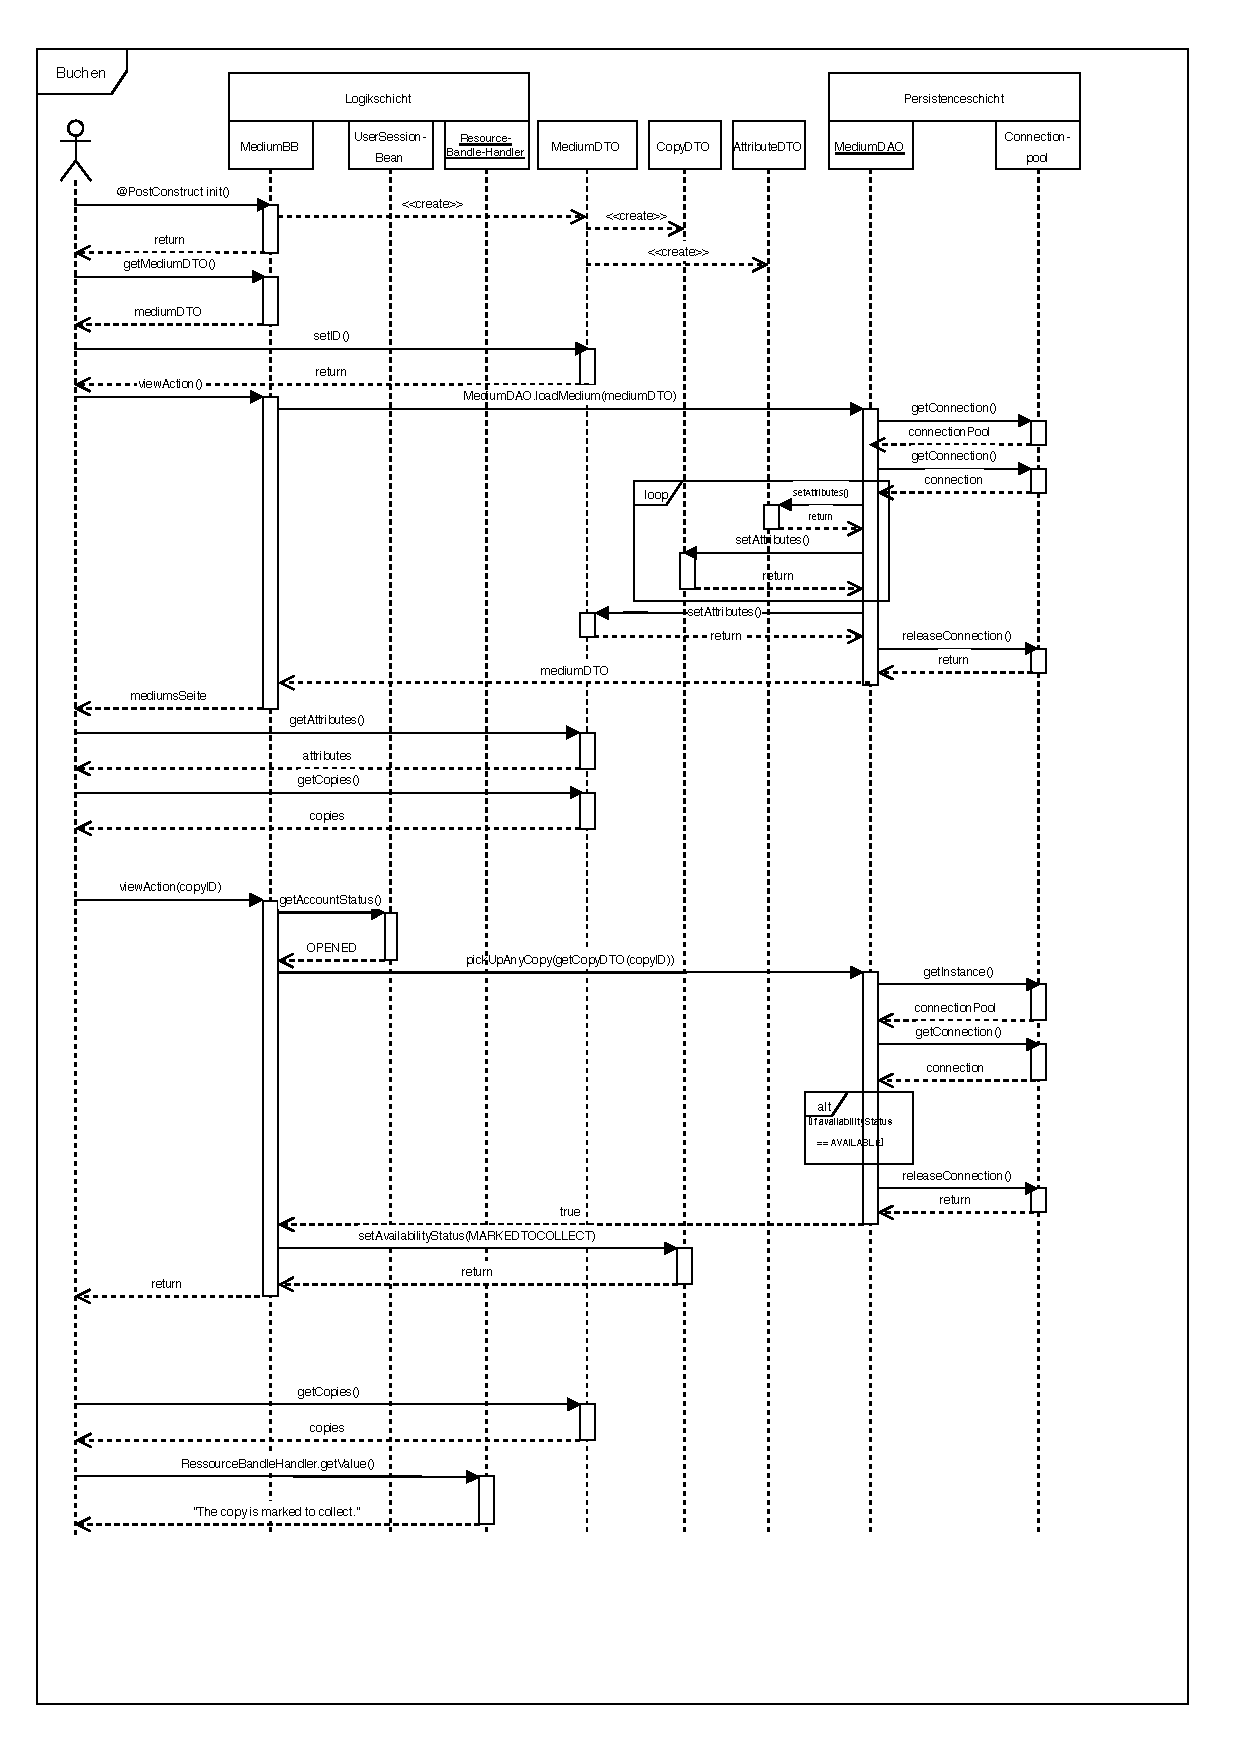
\includegraphics[width = 50em]{Sequenzdiagramm-success-v3.2}
    \caption{Interaktionen beim erfolgreichen Buchen eines Medium-Exemplars}
    \label{Sequenzdiagramm}
\end{figure}
\restoregeometry

\subsection{Interaktionen beim Buchen eines Medium-Exemplars mit fehlender Datenbankverbindung}
\subsubsection{Initialisierung der Mediumsseite}
Beim Laden der Mediumsseite wird zuerst die Methode 'init' als @PostConstruct aufgerufen. Die 'init'-Methode erzeugt ein Medium-DTO, das Medium-DTO hat eine Kollektion der CopyDTOs und eine Kollektion der AttributeDTOs, folglich werden sie vom Medium-DTO erstellt. Der Nutzer bekommt das MediumDTO und setzt eine Medium-ID, die aus dem 'viewParam' zur Verfügung gestellt wird. Danach wird die 'viewAction()' durchgeführt, welche die Mediumsseite durch die statische Methode aus dem Medium-DAO liefern muss. Das Medium-DAO bekommt durch die Methoden 'getInstance()' und 'getConnection()' auf der Persistence-Schicht eine Verbindung von der Singleton-ConnectionPool-Klasse. Aufgrund der fehlenden Verbindung mit der Datenbank kann das Medium-DAO keine SELECT-Anfrage durchführen, deshalb bekommt das Medium-DAO einen SQL-Exception. Das Medium-DAO wandelt den SQL-Exception in den DataAccess-Exception um, danach gibt das Medium-DAO eine Verbindung durch die Methode 'releaseConnection' frei. Im nächsten Schritt wirft das MediumDAO einen Data-Access-Exception in den Medium-BB ein. Der Nutzer ruft die Methode 'handle' des ExceptionHandlers auf; der ExceptionHandler gibt den Fehler durch die Methoden 'getInstance()' und 'addValue(Data-Access-Exception)' in die Singleton-Logger-Klasse ein. Danach bekommt der ExceptionHandler eine Message vom Resource-Bandle-Handler und setzt diese Message in die ErrorBB-Klasse ein. 
\subsubsection{Weiterleitung zur Fehlerseite}
Als Ergebnis der Methode 'handle' liefert der ExceptionHandler dem Nutzer den Link zur Fehlerseite. Das Laden der Fehlerseite wird auf dem Sequenzdiagramm nicht abgebildet.

\newpage

\newgeometry{left=0cm,right=0cm,top=0cm,bottom=2cm}

\begin{figure}[h]
	\hypertarget{Fehlersequenz}{}
    \centering
    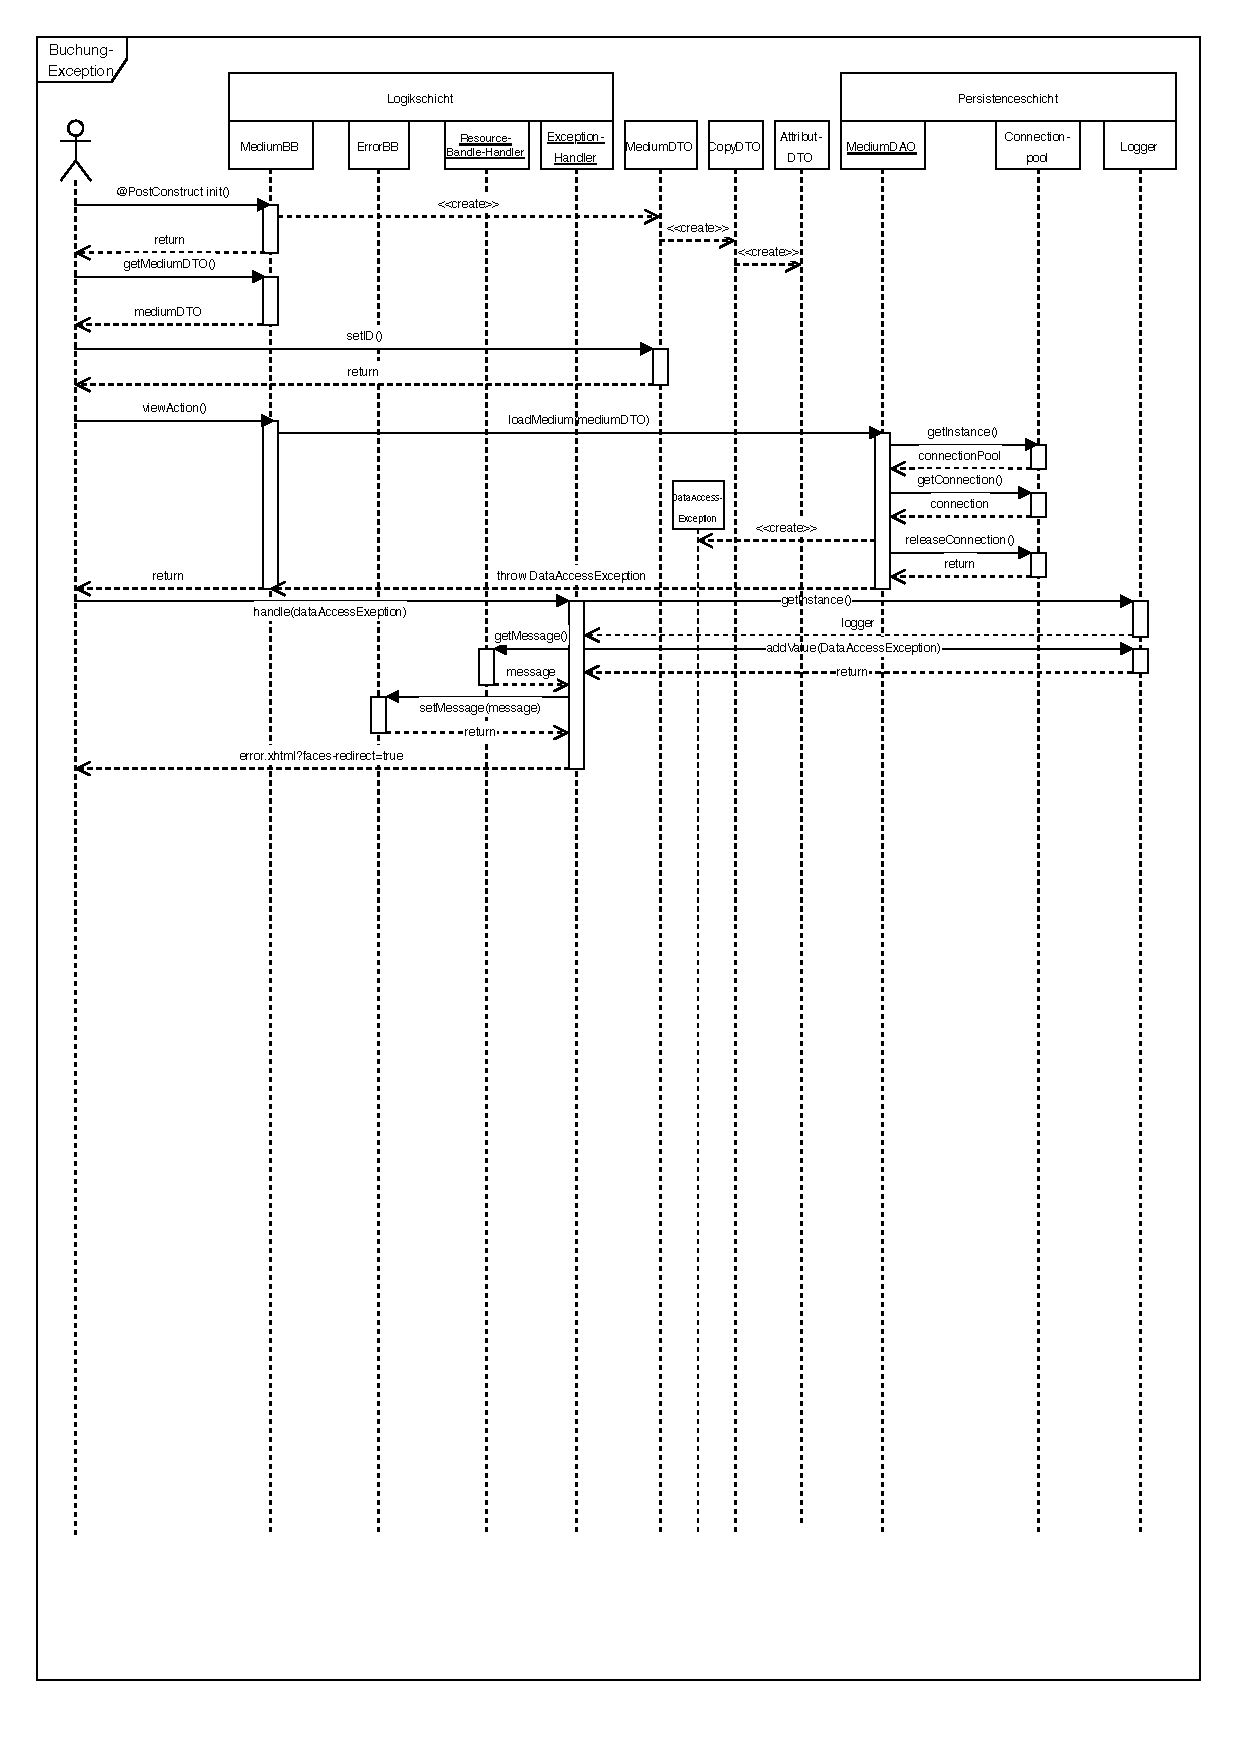
\includegraphics[width = 50em]{Sequenzdiagramm-exception-v4.1}
    \caption{Interaktionen beim Buchen eines Medium-Exemplars mit fehlender Datenbankverbindung}
    \label{Sequenzdiagramm}
\end{figure}

\restoregeometry
\newpage

%----------------------------------------------------------------------Kapitel 9--------------------------------------------------------------------------------------------


\end{document}
